\documentclass[12pt, letterpaper]{article} 

\usepackage{amsmath, amssymb, amsthm, enumerate, graphicx}

\title{MATH 189 HW 7}
\author{Dani Nguyen}
\date{Winter 2026}

\begin{document}
\maketitle
\graphicspath{ {./} }

\noindent \textbf{Question 1}
\begin{enumerate}[a.]
    \item 
\includegraphics[scale=0.8]{1a.png}
    \item Using \texttt{np.random.choice()}, we get \quad
    \begin{tabular}{c | c | c}
        X1 & X2 & Y \\
        \hline
        1 & 4 & blue \\
        1 & 3 & red \\
        0 & 4 & red \\
        5 & 1 & blue \\
        6 & 2 & blue \\
        4 & 0 & red \\
    \end{tabular}
    \item 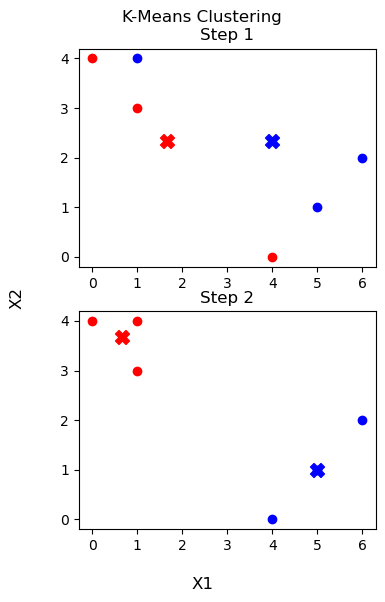
\includegraphics[scale=1.2]{1bcdef.png}
\end{enumerate}
\newpage
\noindent \textbf{Question 2} \\

\noindent \textbf{Question 3} \\

\end{document}